\subsection{\label{subsecResonances}Resonances}

The \kstar\ and $\phi$-mesons are reconstructed at mid 
rapidity $|y|$ $<$ 0.5 via their hadronic decay channels into charged particles, 

\begin{center}
\begin{tabular*}{0.7\textwidth}{rll@{\extracolsep{2cm}}l}
  \kstar & $\to$ & $\pi^{\pm}$ + $K^{\mp}$ & {\footnotesize B.R. = ($\sim$66.6) \%} \\
  $\phi$ & $\to$ & $K^{+}$ + $K^{-}$ & {\footnotesize B.R. = (48.9 $\pm$ 0.5) \%} \\
\end{tabular*}
\end{center}

Both the TPC and TOF information are used to identify charged particles as 
pions or kaons from \kstar\ decays whereas only TPC information is used to identify charged particles as 
kaons from decays of $\phi$-mesons, as in the latter case the combinatorial background is significantly 
smaller.

% The unlike-sign kaons and pions are paired for \kstar\ and unlike-sign 
%kaons are paired for $\phi$-meson to construct the same-event unlike-sign invariant mass distribution. 
%Unlike-sign charged particle tracks satisfying the appropriate TPC and TOF identification criteria are combined into \kstar\ and $\phi$ decay candidates. 
Pairs of pions and kaons (pairs of kaons) of opposite charge are considered to obtain the invariant mass distribution of \kstar\ ($\phi$) decay candidates. An event mixing 
technique is used to estimate the combinatorial background. The mixed-event distribution is 
normalized in the mass region outside of the mass peak, ${\it{i.e}}$ at 1.1 $<$ $M_{\pi\mathrm{K}}$ (GeV/$c^{2}$) 
$<$ 1.15 and 1.035 $<$ $M_{\mathrm{KK}}$ (GeV/$c^{2}$) $<$ 1.045  for \kstar\ and $\phi$-mesons, 
respectively. The normalized mixed-event distribution is subtracted from the same event unlike-sign 
distribution to isolate the relevant signals. 
After mixed-event background subtraction, each invariant mass distribution is fitted with a Breit-Wigner function (Voigtian function) for the signal and a 2nd-order polynomial for any residual background. The parameterizations for the signal are given in Eq.~\ref{kstarfitfun} for the \kstar\ and Eq.~\ref{phifitfun} for the $\phi$-meson:
%The combinatorial 
%background subtracted invariant-mass distributions are fitted using a combined function to 
%describe the signal peak (Breit-Wigner function shown in Eq.~\ref{kstarfitfun}) and residual 
%background (2$^{nd}$ order polynomial) for \kstar\ resonance. For $\phi$-meson a Voigtian function 
%(convolution of Breit-Wigner function and Gaussian, shown in eqn. \ref{phifitfun}), and a residual
%background (2$^{nd}$ order polynomial) is used to fit the invariant-mass distributions. 

\begin{equation}
      \frac{\mathrm{d}N}{\mathrm{d}M_{\pi \mathrm{K}}} = \frac{Y}{2\pi}
      \times \frac{\Gamma} {(M_{\pi \mathrm{K}} - M_0)^{2} + \frac{\Gamma^{2}}{4}}      
      \label{kstarfitfun}
\end{equation}

\begin{equation}
\frac{\mathrm{d}N}{\mathrm{d}M_\mathrm{KK}} = \frac{Y}{2\pi}\int \frac{\Gamma}
     {(M_ \mathrm{KK}-m^{'})^2+\Gamma^2/4}\times\frac{e^{{-(m^{'} -M_{0})}^{2}/2\sigma^2}}{\sqrt{2\pi}\sigma} dm^{'}
     \label{phifitfun}
\end{equation}

where $M_{\pi\mathrm{K}}$ and $M_{\mathrm{KK}}$ are the reconstructed invariant masses of \kstar\
and $\phi$-meson candidates, $M_{0}$, $\Gamma$ and $Y$ are the mass, width and raw yield of the resonances, respectively. The parameter $\sigma$ represents the mass resolution. Figure \ref{fig:KstarPhiSig} shows the invariant mass of $\pi$K (KK) in the left (right) panel 
for 2 $<$ \pt\ $<$ 2.5 GeV/$c$ in the V0M event multiplicity class I.

\begin{figure*}[h]
  %\begin{flushleft}
  %\center{
  %
\includegraphics[width=8cm,height=8cm]{../../SQM2016/figs/resonances_invmass/InvMassKstar_pp7TeV_V0M_I_pT_2to2_5.pdf}
    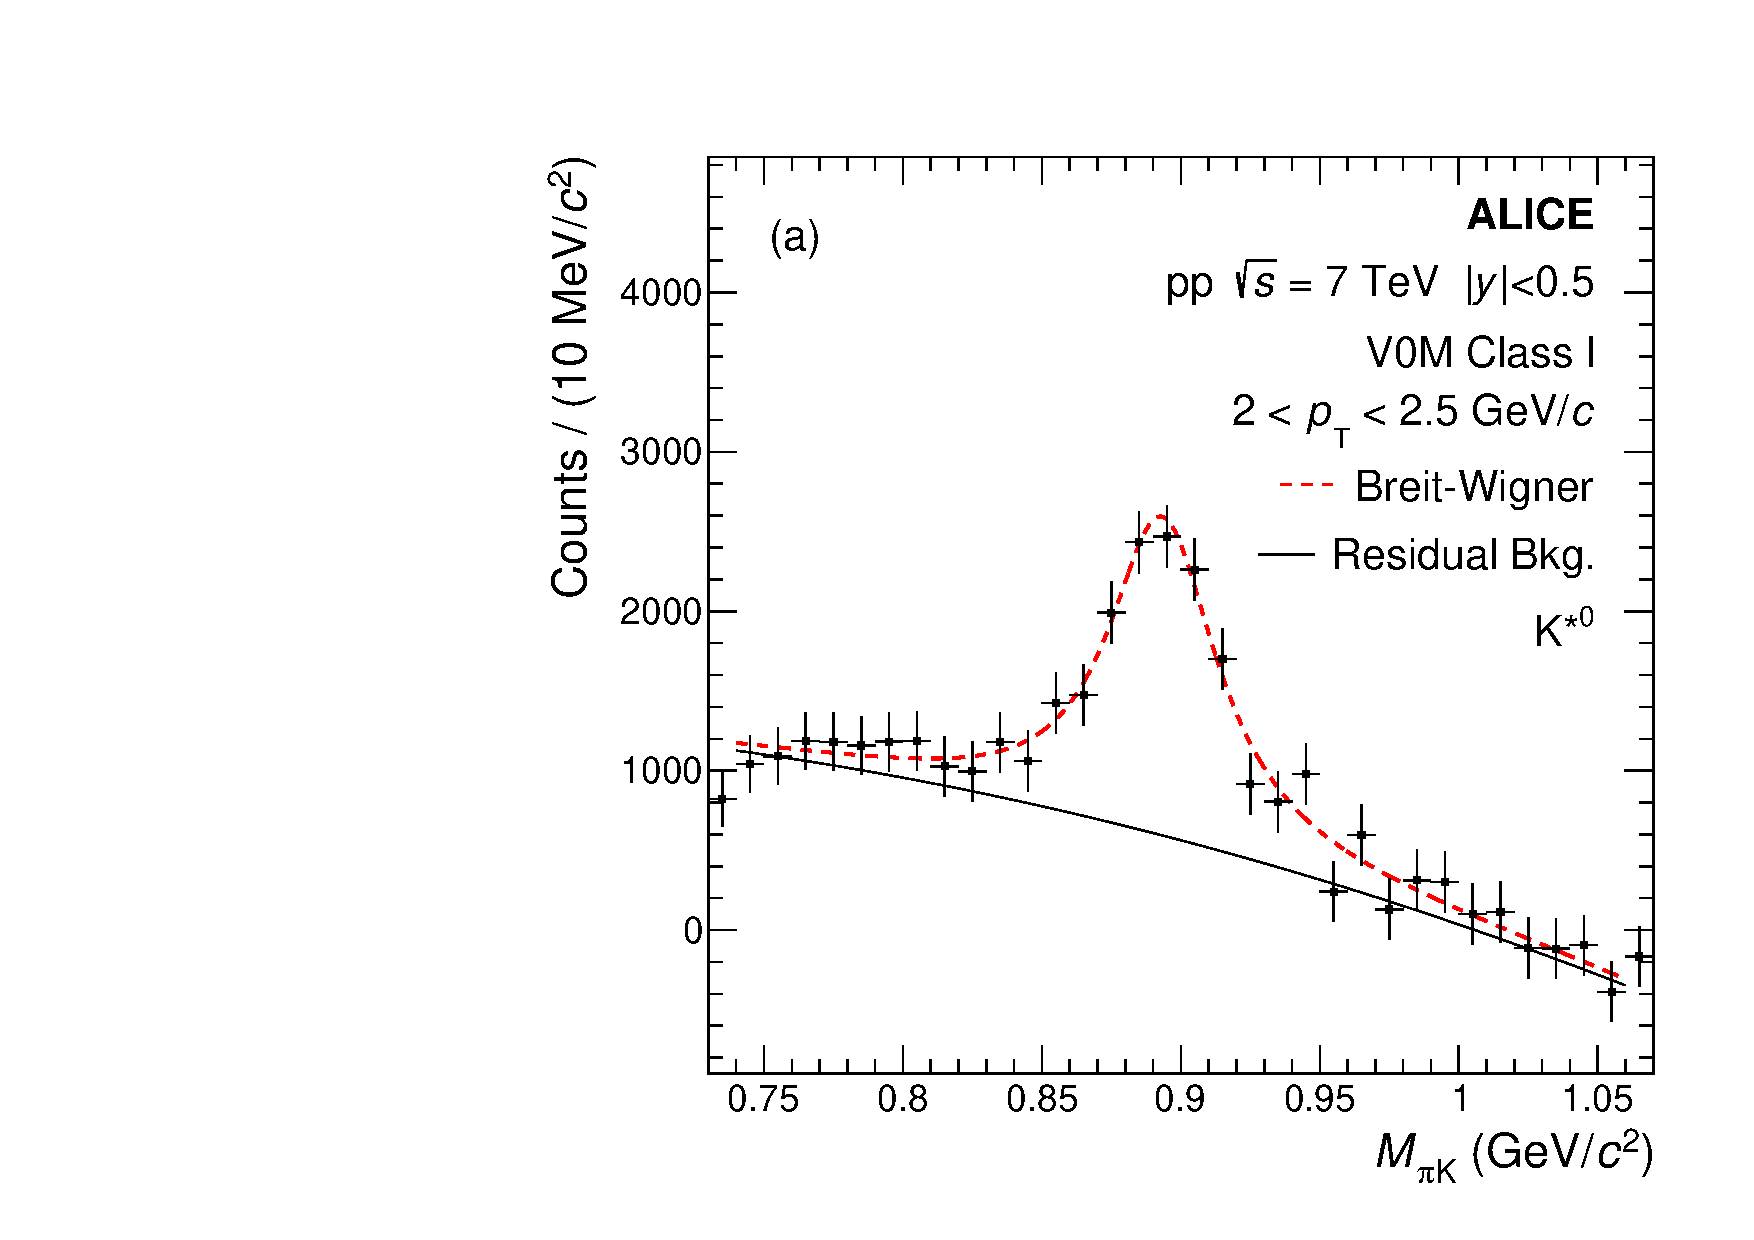
\includegraphics[width=8cm,height=8cm]{figures/InvMassKstar_pp7TeV_V0M_I_pT_2to2_5.pdf}
  %\center{
  %
\includegraphics[width=8cm,height=8cm]{../../SQM2016/figs/resonances_invmass/InvMassPhi_pp7TeV_V0M_I_pT_2to2_5.pdf}
    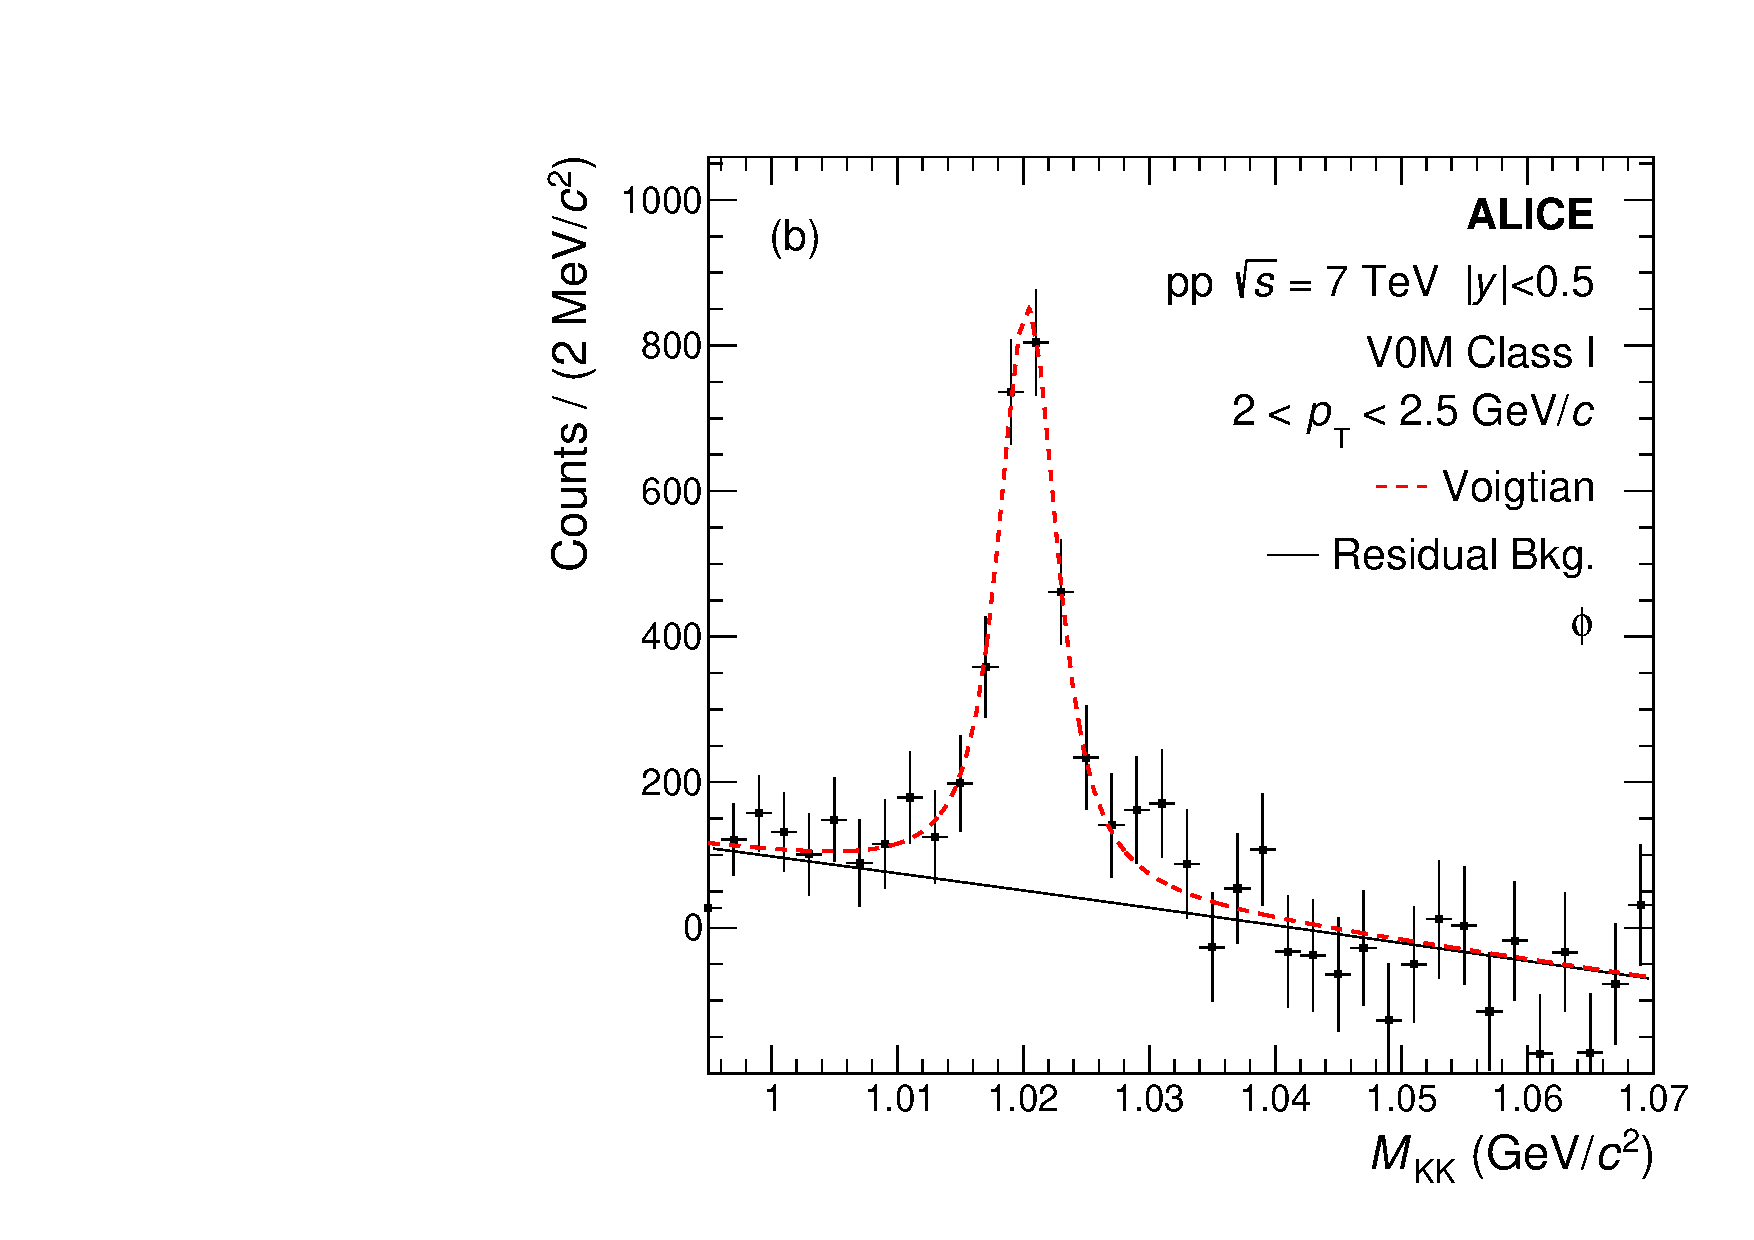
\includegraphics[width=8cm,height=8cm]{figures/InvMassPhi_pp7TeV_V0M_I_pT_2to2_5.pdf}
  %\end{flushleft}
  \caption{Invariant mass distributions of $\pi$K and KK in the momentum range of 2 $<$ \pt\ 
    $<$ 2.5 GeV/$c$ for V0M event multiplicity class I are 
    shown in panels (a) and (b), respectively. The statistical uncertainties are shown by vertical bars. The red dashed 
    curves represent fits to the distributions and the solid curves describe the residual
    background.}
  \label{fig:KstarPhiSig}
\end{figure*}

The raw yields are extracted in each \pt\ bin and event multiplicity interval as done in previous 
works~\cite{Abelev:2012hy,Adam:2016bpr,Abelev:2014uua}. In this analysis, detector 
acceptance and reconstruction efficiency are re-weighted in each 
\pt\ bin to take into account the differences between generated and real data spectral shapes.
  
The sources of systematic uncertainties for \kstar\ and $\phi$-meson production in pp collisions 
are the TPC-ITS matching efficiency, track selection criteria, PID, yield extraction method, hadronic 
interaction and material budget, and were evaluated following the same prescription used in previous 
works~\cite{Adam:2016bpr, Abelev:2012hy}. 
The main source of uncertainty for \kstar\ and $\phi$ comes from 
the determination of the TPC-ITS track matching efficiency. This contribution has been estimated 
to be a \pt-independent effect of 3$\%$ for charged particles~\cite{id2208submitted}, which 
results in a 6\% effect when 
any two primary tracks are combined in the invariant mass analysis of \kstar\ and $\phi$. For both \kstar\ 
and $\phi$, the uncertainties due to various track selection cuts from low to high-\pt\ are found 
to be 0.9-3.0\% and 1.6-2.4\%, respectively. The systematic uncertainty due to the signal extraction 
 includes variations in the fit range, fit function and normalization range and is of $\sim$5-10\% 
($\sim$3-9\%) from low to high \pt\ for \kstar\ ($\phi$). The uncertainty due to different PID selection methods
is estimated to be $\sim$2-4\% ($\sim$1-2$\%$) for  \kstar\ ($\phi$). The knowledge of the material budget 
for both \kstar\ and $\phi$ contributes to $\sim$4\% and $\sim$6\% at low \pt\ and is negligible at high \pt. 
The contribution from the estimate of the hadronic interaction cross section in the 
detector material at low-\pt\ is $\sim$4\% ($\sim$6\%) for \kstar\ ($\phi$) and negligible at high-\pt. The 
total systematic uncertainty for \kstar and $\phi$ is estimated to be about 12\% and 10\%, 
respectively. The maximum value of the multiplicity-independent systematic uncertainty is found 
to be $\sim$8\% ($\sim$5\%) for \kstar\ ($\phi$). The main contributions to the systematic 
uncertainties are summarized in Tab. \ref{tab:sysresonances}.
    
The systematic uncertainties were studied independently for all event classes, in order to separate the sources 
that are multiplicity-dependent and uncorrelated across multiplicity bins. In particular, signal 
extraction and PID are fully uncorrelated sources, whereas global tracking, track cuts, material 
budget and hadronic cross sections are correlated among different event multiplicity classes.

%Table with systematics: this is a tentative inclusion, to be worked out! 
\begin{table*}[h]
  \begin{tabularx}{\linewidth}{l*{3}{Y}*{3}{Y}}
\hline\hline
\vspace{0.1cm}
    Hadron species &  \multicolumn{3}{c}{\kstar} & \multicolumn{3}{c}{$\phi$} \\
    \pt (\GeVc)       &   0.4 & 3.0 & 10.0 &   0.6 & 3.0 & 10.0  \\
% Not obvious: would we prefer quoting only 2 and not 3 pt ranges here? 
% --- it might depend on the pT dendence of these systematics 
 %   PID technique  &   TPC-TOF & No PID & \multicolumn{2}{c}{TPC-TOF} \\
    \cmidrule(lr){2-4} \cmidrule(lr){5-7} 
    Global tracking efficiency & \multicolumn{3}{c}{6} & \multicolumn{3}{c}{6} \\
    Signal extraction &5.1&   4.6&   9.7&   3.1&   3.2&   8.5 \\ 
    Track selection cuts &    3.0 &  2.1 & 0.9 &  1.6 &   1.6 &  2.4  \\
    Particle identification & 1.8 & 2.5 &  4.0 &   1.1  & 1.9  &  2.1 \\ 
    Material budget     & 4.3 &  0.8 &  0.1 &  6.2 &   0.4 &    - \\ 
    Hadronic interactions & 1.9 &0.9 & 0.1 & 1.4 & 0.7 & - \\
    \cmidrule(lr){2-4} \cmidrule(lr){5-7} 
    Total & 9.8&  8.3&  12.1&  9.5& 7.3&    9.0 \\ 
    Total ($N_{ch}$-independent) & 7.7&6.6&8.1 & 3& 5&5 \\ 
\hline\hline
  \end{tabularx}
  \newline
    \caption{Main sources and values of the relative systematic uncertainties (expressed in \%) of the \pt-differential yields of $\phi$ and \kstar\ resonances. The values are reported for low, intermediate and high \pt. The The contributions that act differently in the various event classes are removed from the total (quadratic sum of all contributions), defining the $N_{ch}$-independent ones, which are correlated across different multiplicity intervals. }
  \label{tab:sysresonances}  
\end{table*}

